\documentclass{beamer}

% Required packages
\usepackage{xcolor}
\usepackage{tikz}
\usepackage{amsmath}
\usepackage{array}
\usepackage{listings}

% Define custom DS9-inspired colors
\definecolor{ds9blue}{RGB}{25,25,112}    % Midnight Blue
\definecolor{ds9gold}{RGB}{218,165,32}   % Goldenrod
\definecolor{ds9grey}{RGB}{105,105,105}  % Dim Gray
\definecolor{ds9red}{RGB}{178,34,34}     % Firebrick

% Configure listings for code blocks
\lstset{
  basicstyle=\ttfamily\small,
  columns=flexible,
  breaklines=true,
  frame=single,
  xleftmargin=0.1\textwidth,
  xrightmargin=0.1\textwidth
}

% Use Madrid theme with custom colors
\usetheme{Madrid}

% Customize colors
\setbeamercolor{structure}{fg=ds9blue}
\setbeamercolor{title}{fg=ds9blue, bg=ds9gold!15}
\setbeamercolor{frametitle}{fg=ds9blue, bg=ds9gold!15}
\setbeamercolor{block title}{bg=ds9blue, fg=white}
\setbeamercolor{block body}{bg=ds9blue!10}
\setbeamercolor{item}{fg=ds9blue}
\setbeamercolor{alerted text}{fg=ds9red}
\setbeamercolor{example text}{fg=ds9blue}

% Title page information
\title[2D Arrays]{PHYS11 CH: Two Dimensional Arrays}
\subtitle{Data Structures and Memory Organization}
\author[Mr. Gullo]{Mr. Gullo}
\date[Feb 2025]{February 25, 2025}
\institute{Computer Science Department}

\begin{document}

% Title frame
\begin{frame}
    \titlepage
\end{frame}

% Table of contents
\begin{frame}{Outline}
    \tableofcontents
\end{frame}

\section{Introduction to Two Dimensional Arrays}

\begin{frame}{Learning Objectives}
    \begin{block}{By the end of this lesson, you will be able to:}
        \begin{itemize}
            \item Define and declare two-dimensional arrays in C++
            \item Understand how 2D arrays are represented in memory
            \item Access and manipulate elements in a 2D array
            \item Implement functions that work with 2D arrays
            \item Solve problems using 2D arrays
        \end{itemize}
    \end{block}
\end{frame}

\begin{frame}{One Dimensional Arrays - Review}
    \begin{columns}
        \begin{column}{0.5\textwidth}
            \begin{block}{Declaration}
                \begin{lstlisting}
int arr[6];
                \end{lstlisting}
            \end{block}
        \end{column}
        \begin{column}{0.5\textwidth}
            \begin{block}{Memory Representation}
                \begin{lstlisting}
+--------+--------+--------+--------+--------+--------+
| arr[0] | arr[1] | arr[2] | arr[3] | arr[4] | arr[5] |
+--------+--------+--------+--------+--------+--------+
                \end{lstlisting}
            \end{block}
        \end{column}
    \end{columns}
    
    \begin{itemize}
        \item A one-dimensional array stores elements in a single row
        \item Each element is accessed with a single index
        \item Elements are stored contiguously in memory
    \end{itemize}
\end{frame}

\begin{frame}{Two Dimensional Arrays}
    \begin{columns}
        \begin{column}{0.5\textwidth}
            \begin{block}{Declaration}
                \begin{lstlisting}
int arr[3][6];
                \end{lstlisting}
            \end{block}
            \vspace{0.5cm}
            We can think of this as:
            \begin{itemize}
                \item 3 rows of arrays
                \item Each row contains 6 elements
                \item Total of $3 \times 6 = 18$ elements
            \end{itemize}
        \end{column}
        \begin{column}{0.5\textwidth}
            \begin{block}{Memory Representation}
                \begin{lstlisting}[basicstyle=\ttfamily\footnotesize]
Memory layout (row-major order):
arr[0][0] arr[0][1] arr[0][2] arr[0][3] arr[0][4] arr[0][5]
arr[1][0] arr[1][1] arr[1][2] arr[1][3] arr[1][4] arr[1][5]
arr[2][0] arr[2][1] arr[2][2] arr[2][3] arr[2][4] arr[2][5]
                \end{lstlisting}
            \end{block}
        \end{column}
    \end{columns}
\end{frame}

\begin{frame}{Accessing 2D Array Elements}
    \begin{itemize}
        \item Elements are accessed using two indices: [row][column]
        \item The first index (row) ranges from 0 to rows-1
        \item The second index (column) ranges from 0 to columns-1
    \end{itemize}
    
    \begin{exampleblock}{Example}
        For \texttt{arr[3][6]}:
        \begin{itemize}
            \item Valid indices range from [0][0] to [2][5]
            \item \texttt{arr[1][4]} accesses the element in the 2nd row, 5th column
            \item \texttt{arr[0][2] = 42;} assigns the value 42 to the element in the 1st row, 3rd column
        \end{itemize}
    \end{exampleblock}
    
    \begin{alertblock}{Be Careful!}
        \texttt{arr[3][6]} is an out-of-bounds access and will lead to undefined behavior!
    \end{alertblock}
\end{frame}

\section{Limitations and Function Parameters}

\begin{frame}{Limitations of 2D Arrays in C++}
    \begin{alertblock}{Important Limitation}
        When passing 2D arrays to functions, you \textbf{must} specify the number of columns!
    \end{alertblock}
    
    \begin{columns}
        \begin{column}{0.45\textwidth}
            \begin{block}{\textcolor{ds9red}{Invalid}}
                \begin{lstlisting}
int someFunction(int arr[][]);
                \end{lstlisting}
            \end{block}
        \end{column}
        \begin{column}{0.45\textwidth}
            \begin{block}{\textcolor{ds9blue}{Valid}}
                \begin{lstlisting}
int someFunction(int arr[][COLS]);
                \end{lstlisting}
            \end{block}
        \end{column}
    \end{columns}
    
    \begin{itemize}
        \item The number of columns must be a constant value
        \item The first dimension (rows) can be unspecified
        \item Typically, use a global constant or \#define for COLS
    \end{itemize}
\end{frame}

\begin{frame}{Function Parameter Syntax}
    \begin{exampleblock}{Function Declaration Examples}
        \begin{lstlisting}
// Prints a 2D array
void printArr2d(int arr[][NUM_COLS], int rows);

// Calculates the sum of elements in a specific row
int rowSum(int arr[][NUM_COLS], int rowNum);

// Finds the maximum value in a specific row
int rowMax(int arr[][NUM_COLS], int rowNum);

// Finds the row with the largest sum
int maxRowSum(int arr[][NUM_COLS], int rows);
        \end{lstlisting}
    \end{exampleblock}
\end{frame}

\section{Operations on 2D Arrays}

\begin{frame}{Printing a 2D Array}
    \begin{columns}
        \begin{column}{0.48\textwidth}
            \begin{block}{Function Declaration}
                \begin{lstlisting}[basicstyle=\ttfamily\footnotesize]
void printArr2d(int arr[][NUM_COLS], 
                int rows);
/*
 Parameters: 
 arr, a 2D array of size rows x cols
 Behavior: 
 uses cout to output the array 
 columns as a comma separated 
 list for each row
*/
                \end{lstlisting}
            \end{block}
        \end{column}
        \begin{column}{0.48\textwidth}
            \begin{block}{Implementation}
                \begin{lstlisting}[basicstyle=\ttfamily\footnotesize]
void printArr2d(int arr[][NUM_COLS], 
                int rows) {
  for (int i = 0; i < rows; i++) {
    cout << "Row " << i << ": ";
    for (int j = 0; j < NUM_COLS; j++) {
      cout << arr[i][j];
      if (j < NUM_COLS - 1) 
        cout << ", ";
    }
    cout << endl;
  }
}
                \end{lstlisting}
            \end{block}
        \end{column}
    \end{columns}
\end{frame}

\begin{frame}{Calculating Row Sum}
    \begin{columns}
        \begin{column}{0.48\textwidth}
            \begin{block}{Function Declaration}
                \begin{lstlisting}[basicstyle=\ttfamily\footnotesize]
int rowSum(int arr[][NUM_COLS], 
           int rowNum);
/*
 Finds the sum of the 
 elements of rowNum
 Parameters:
 arr[][NUM_COLS] - array with 
 at least rowNum+1 rows
 rowNum - the row to find 
 the sum from 0 to number 
 of rows - 1
*/
                \end{lstlisting}
            \end{block}
        \end{column}
        \begin{column}{0.48\textwidth}
            \begin{block}{Implementation}
                \begin{lstlisting}[basicstyle=\ttfamily\footnotesize]
int rowSum(int arr[][NUM_COLS], 
           int rowNum) {
  int sum = 0;
  
  for (int j = 0; j < NUM_COLS; j++) {
    sum += arr[rowNum][j];
  }
  
  return sum;
}
                \end{lstlisting}
            \end{block}
        \end{column}
    \end{columns}
\end{frame}

\begin{frame}{Finding Row Maximum}
    \begin{columns}
        \begin{column}{0.48\textwidth}
            \begin{block}{Function Declaration}
                \begin{lstlisting}[basicstyle=\ttfamily\footnotesize]
int rowMax(int arr[][NUM_COLS], 
           int rowNum);
/*
 Finds the largest element 
 in the rowNum row
 Parameters:
 arr[][NUM_COLS] - array with 
 at least rowNum+1 rows
 rowNum - the row to find largest
 value in the rowNum row
 Note: rows are from 0 to 
 number of rows - 1
*/
                \end{lstlisting}
            \end{block}
        \end{column}
        \begin{column}{0.48\textwidth}
            \begin{block}{Implementation}
                \begin{lstlisting}[basicstyle=\ttfamily\footnotesize]
int rowMax(int arr[][NUM_COLS], 
           int rowNum) {
  int max = arr[rowNum][0];
  
  for (int j = 1; j < NUM_COLS; j++) {
    if (arr[rowNum][j] > max) {
      max = arr[rowNum][j];
    }
  }
  
  return max;
}
                \end{lstlisting}
            \end{block}
        \end{column}
    \end{columns}
\end{frame}

\begin{frame}{Finding Maximum Row Sum}
    \begin{columns}
        \begin{column}{0.48\textwidth}
            \begin{block}{Function Declaration}
                \begin{lstlisting}[basicstyle=\ttfamily\footnotesize]
int maxRowSum(int arr[][NUM_COLS], 
              int rows);
/*
 Finds the largest row sum
 Parameters:
 arr[][NUM_COLS] - 2D array of 
 size rows*NUM_COLS
 row- the total number of rows
*/
                \end{lstlisting}
            \end{block}
        \end{column}
        \begin{column}{0.48\textwidth}
            \begin{block}{Implementation}
                \begin{lstlisting}[basicstyle=\ttfamily\footnotesize]
int maxRowSum(int arr[][NUM_COLS], 
              int rows) {
  int maxSum = rowSum(arr, 0);
  
  for (int i = 1; i < rows; i++) {
    int currentSum = rowSum(arr, i);
    if (currentSum > maxSum) {
      maxSum = currentSum;
    }
  }
  
  return maxSum;
}
                \end{lstlisting}
            \end{block}
        \end{column}
    \end{columns}
\end{frame}

\section{The Treasure Map Problem}

\begin{frame}{Treasure Map Problem}
    \begin{block}{Problem Description}
        Given a grid (2D array) of numbers representing treasures:
        \begin{itemize}
            \item Start at any cell in the top row
            \item Move down, but can only move to one of the three adjacent cells in the next row
            \item End at any cell in the bottom row
            \item Find the path with the maximum treasure sum
        \end{itemize}
    \end{block}
    
    \begin{lstlisting}[basicstyle=\ttfamily\small]
+---+---+---+---+---+
| 8 | 9 | 6 | 8 | 2 |
+---+---+---+---+---+
| 1 | 8 | 7 | 6 | 3 |
+---+---+---+---+---+
| 5 | 3 | 1 |10 | 5 |
+---+---+---+---+---+
| 9 | 6 | 8 | 4 | 9 |
+---+---+---+---+---+
| 7 | 1 | 9 | 7 | 7 |
+---+---+---+---+---+
| 7 | 9 | 5 | 9 | 8 |
+---+---+---+---+---+
    \end{lstlisting}
\end{frame}

\begin{frame}{Movement Rules in Treasure Map}
    \begin{columns}
        \begin{column}{0.6\textwidth}
            \begin{block}{Rules for Movement}
                \begin{itemize}
                    \item Start at any cell in the top row
                    \item From a cell [i][j], can move to:
                    \begin{itemize}
                        \item [i+1][j-1] (diagonal left)
                        \item [i+1][j] (directly below)
                        \item [i+1][j+1] (diagonal right)
                    \end{itemize}
                    \item If at edge, can't move diagonally outside grid
                    \item End at any cell in the bottom row
                \end{itemize}
            \end{block}
        \end{column}
        \begin{column}{0.4\textwidth}
            \begin{center}
                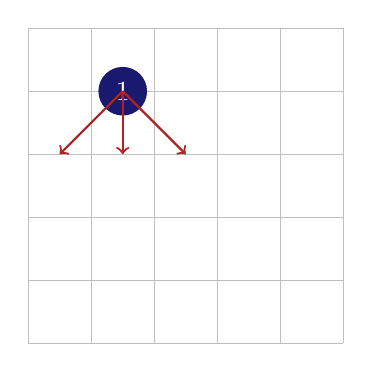
\begin{tikzpicture}
                    \draw[step=0.8cm,color=gray!50] (0,0) grid (4,4);
                    \node[circle,fill=ds9blue,text=white] at (1.2,3.2) {1};
                    \draw[->,thick,color=ds9red] (1.2,3.2) -- (0.4,2.4);
                    \draw[->,thick,color=ds9red] (1.2,3.2) -- (1.2,2.4);
                    \draw[->,thick,color=ds9red] (1.2,3.2) -- (2.0,2.4);
                \end{tikzpicture}
            \end{center}
        \end{column}
    \end{columns}
\end{frame}

\begin{frame}{Maximum Path Solution}
    \begin{columns}
        \begin{column}{0.5\textwidth}
            \begin{lstlisting}[basicstyle=\ttfamily\small]
+---+---+---+---+---+
| 8 |*9*| 6 | 8 | 2 |  * = Path
+---+---+---+---+---+
| 1 | 8 |*7*| 6 | 3 |
+---+---+---+---+---+
| 5 | 3 | 1 |*10*| 5 |
+---+---+---+---+---+
| 9 | 6 |*8*| 4 | 9 |
+---+---+---+---+---+
| 7 | 1 |*9*| 7 | 7 |
+---+---+---+---+---+
| 7 |*9*| 5 | 9 | 8 |
+---+---+---+---+---+
            \end{lstlisting}
            \begin{center}
                Maximum Path: 9 + 7 + 10 + 8 + 9 + 9 = 52
            \end{center}
        \end{column}
        \begin{column}{0.5\textwidth}
            \begin{block}{Dynamic Programming Approach}
                \begin{itemize}
                    \item Start with the top row (base case)
                    \item For each row, calculate cumulative sums
                    \item At each cell, choose the maximum of three possible paths from above
                    \item Continue until we reach the bottom row
                    \item Find the maximum value in the bottom row
                \end{itemize}
            \end{block}
        \end{column}
    \end{columns}
\end{frame}

\begin{frame}{Cumulative Sums Calculation}
    \begin{columns}
        \begin{column}{0.5\textwidth}
            \begin{lstlisting}[basicstyle=\ttfamily\footnotesize]
+------+------+-----+-----+-----+
|  8   |  9   |  6  |  8  |  2  |
+------+------+-----+-----+-----+
| 1+9  | 8+9  | 7+9 | 6+8 | 3+8 |
+------+------+-----+-----+-----+
| 5+17 | 3+17 | 18  | 26  | 19  |
+------+------+-----+-----+-----+
|  31  |  28  | 34  | 30  | 35  |
+------+------+-----+-----+-----+
|  38  |  35  | 43  | 42  | 42  |
+------+------+-----+-----+-----+
|  45  |  52  | 48  | 52  | 50  |
+------+------+-----+-----+-----+
            \end{lstlisting}
        \end{column}
        \begin{column}{0.5\textwidth}
            \begin{block}{Calculation Method}
                For each cell [i][j] (except first row):
                \begin{align*}
                sum[i][j] = arr[i][j] + max(&sum[i-1][j-1], \\
                                        &sum[i-1][j], \\
                                        &sum[i-1][j+1])
                \end{align*}
                
                With boundary checks for edges.
            \end{block}
        \end{column}
    \end{columns}
\end{frame}

\begin{frame}{Summary}
    \begin{block}{Key Concepts}
        \begin{itemize}
            \item Two-dimensional arrays store data in a grid-like structure
            \item Accessed using two indices: [row][column]
            \item When passing to functions, column size must be specified
            \item Common operations:
            \begin{itemize}
                \item Traversing row by row
                \item Finding row sums and maximums
                \item Dynamic programming for pathfinding problems
            \end{itemize}
        \end{itemize}
    \end{block}
    
    \begin{alertblock}{Remember}
        \begin{itemize}
            \item Valid indices range from [0][0] to [rows-1][cols-1]
            \item Always check array bounds to prevent errors
            \item Use descriptive function parameters for clarity
        \end{itemize}
    \end{alertblock}
\end{frame}

\end{document}